\setchapterpreamble[u]{\margintoc}
\chapter{Performance evaluation in \gls{medLabel} processes: standard methodology proposal}
\labch{solarmed:std}

\tldrbox{
    % This chapter presents a standard method for performance evaluation of \gls{medLabel}
    % processes, which can also be extrapolated to other thermal separation
    % processes. This method considers aspects such as instrumentation
    % requirements, process control, and the adequacy of performance metrics,
    % including uncertainty in their determination. In addition, it has been
    % developed an algorithm for the automatic identification of steady-state
    % operation, which allows to increase the reliability and robustness of
    % evaluations under variable conditions. The experimental results also show
    % that the proposed method is robust and reliable, allowing for a fair
    % comparison of \gls{medLabel} processes under different conditions.

    This chapter presents a standardized method for evaluating the performance of
    \gls{medLabel} processes, which can also be extended to other thermal
    separation technologies. The method addresses key aspects such as
    instrumentation requirements, process control, and the suitability of
    performance metrics, including the uncertainties associated with their
    determination. Additionally, an algorithm has been developed for the automatic
    detection of steady-state operation, enhancing the reliability and robustness
    of evaluations under variable conditions. Experimental results confirm that the
    proposed method is both robust and reliable, enabling fair comparisons of
    \gls{medLabel} processes across different operating scenarios.

    The experimentation includes the evaluation of the process at high
    \glspl{tbtLabel}. The results are analyzed using different performance
    metrics and the scale formation risk is estimated by the
    \fullgls{rsiLabel}. The results show that the \gls{medLabel} process can be operated
    at high \glspl{tbtLabel} without significant scale formation and achieve
    higher concentrations, but without significant improvements in thermal
    performance and limited reconcentration capacity if no changes to its
    design are made. 
}

\section*{Introduction}

The future of \gls{medLabel} in desalination and brine concentration
applications depends on the technical development of the process and its
integration with other
technologies~\sidecite{ghenai_performance_2021,son_pilot_2020}. The performance
of this technology and how it is evaluated plays an important role in this
development.

% Estado del arte
Although efforts have been made to propose performance metrics to evaluate
the multi-effect evaporation process, there is neither consensus in which
metrics are the most suitable~\sidecite{burgess_solar_2000} nor standards on
how to evaluate the experimental process. The only standard existing in
\gls{medLabel} is not related to performance evaluation, but to cost structures
and determinants~\sidecite{pinto_desalination_2017}. 

For the performance
evaluation of \gls{medLabel} processes, originally, the index
\fullgls{gorLabel} was used for plants operating with steam as external energy
source. In order not to be limited to steam-driven systems and to take into
account sensible heat sources, a new performance index was defined: the
\gls{prLabel}~\sidecite{mistry_entropy_2011,el-dessouky_fundamentals_2002}, which is
currently the most widely adopted for \gls{medLabel} performance evaluation
although it is constrained by using a reference enthalpy of 2326 kJ equivalent
to 1000 BTU. In \sidecite{christ_thermodynamic_2014}, a variation of this
metric called the Waste Heat Performance Ratio ($PR_{WH}$) was suggested to
account for the potential of low-grade waste heat sources. Another widespread
thermal performance metric that has been used in \gls{medLabel} is the
\fullgls{stecLabel} and its electrical equivalent, the \fullgls{seecLabel}.
% Limitaciones métricas simples
However, there are certain limitations in the aforementioned metrics that
challenge making a fair comparison between desalination systems that use
different energy sources \ie electrical and thermal\sidenote{the value of 1 kWh
electric differs from that of 1 kWh thermal in terms of their ability to
produce work, as the latter is constrained by the Carnot
efficiency~\cite{lienhard_thermodynamics_2017}}. Furthermore, the ability of
thermal energy to perform work changes with its temperature, so it is essential
to consider the quality of the thermal energy used in desalination processes.
This limitation of traditional energetic metrics was showcased in Bouma et al.
\sidecite{bouma_metrics_2020} where they compared four different configurations
of \gls{medLabel} plants: a low temperature \gls{medLabel} configuration
(LT-MED), a \gls{medLabel} unit incorporating Thermal Vapor Compression
(MED-TVC), a \gls{medLabel} unit using nanofiltration (NF-LT-MED) for feedwater
pretreatment, and a combination of TVC and nanofiltration. Although the
\gls{stecLabel} values favored the use of TVC, a more rigorous %exergetic
analysis revealed that the most efficient systems were those that used lower
temperature heat sources (LT-MED and NF-LT-MED).

%Furthermore, each energy type possesses different thermodynamic or economic
%values, further complicating the evaluation process. It is important to note
%that the value of 1 kWh electric differs from that of 1 kWh thermal in terms
%of their ability to produce work, as the latter is constrained by the Carnot
%efficiency. Consequently, a system that excels according to one metric may do
%so at the expense of the other, and even assessing the same system under
%different conditions can prove difficult. Secondly, the quality of thermal
%energy is not uniform, and its evaluation depends on its temperature-dependent
%thermodynamic properties~\sidecite{darwish_multi-effect_2006}. As the temperature
%of thermal energy rises, its ability to perform work or its availability
%increases, indicating higher exergy or quality. Hence, when assessing the
%practical applications of an \gls{medLabel} system, the quality of thermal energy
%employed becomes a critical factor. 

% Estado del arte de análisis exergéticos. Thermal energy is not a homogeneous
%form of energy, and its quality is determined by its thermodynamic properties,
%which are temperature-dependent~\sidecite{darwishMultieffectBoilingSystems2006}.
%As the temperature of thermal energy increases, so does its ability to do work
%or availability, which is reflected in its higher exergy or quality.
%Therefore, the quality of thermal energy used in an \gls{medLabel} system is a crucial
%factor in evaluating its performance in practical applications. This
%limitation of traditional metrics was showcased in
%\cite{boumaMetricsMatterAccurately2020}, where four \gls{medLabel} plants configurations
%were compared: a basic configuration, one that included Thermal Vapor
%Compression (TVC), one where the feedwater was pretreated with nanofiltration
%(NF) and a combination of both. Even though STEC figures favored the use of
%TVC an exergetic analysis reveals that SEXC values actually fall towards the
%basic \gls{medLabel} or MED-NF. 

Some authors have carried out exergy analyzes to overcome the limitations
aforementioned of energy performance metrics.  Darwish et al.
~\sidecite{darwish_multieffect_2006} proposed two new metrics: Specific Fuel
Energy and Equivalent Specific Work. The first compares the energy used for the
desalination process that could otherwise be used for energy generation in a
turbine for which it was assumed a value for the efficiency of the power plant.
The second sets the work potential of the extracted steam as a baseline,
considering the desalination plant separation efficiency and adding the energy
consumption for pumping. The problem of this study is that it is limited to
cogeneration schemes (joint electricity and water production) and would not be
useful in the case of desalination with low-temperature sources. Shahzad et
al.~\sidecite{shahzad_standard_2019} developed an approach based on the second
law of thermodynamics, which is also useful only for cogeneration schemes. They
proposed a common metric called the Standard Universal Performance Ratio to
compare desalination processes using different kinds of energy, which is based
on conversion of different types and grades of energies to standard primary
energy. In this case, conversion factors were proposed to convert the derived
energy input to the standard primary energy. Other authors have performed
exergy analyses for stand-alone desalination processes, as is the case of
Lienhard et al.~\sidecite{lienhard_thermodynamics_2017} and Brogioli et
al.~\sidecite{brogioli_thermodynamic_2018}, who considered desalination
processes as a black box and the ideal work or the thermodynamic limit for the
separation of dissolved salts in seawater as the Carnot work.

The problem with the exergy analyses is that they are more complex
~\sidecite{spiegler_elsayed_2001} due to the need to consider several aspects
not present in simple energetic metrics: definition of dead state and control
volume~\sidecite{sharqawy_exergy_2011}, chemical exergy modeling of seawater
~\sidecite{sharqawy_formulation_2010, mistry_effect_2012} and minimum energy
reference (least and minimum work of separation)
~\sidecite{mistry_generalized_2013,thiel_energy_2015}. Probably because of
their complexity, they have not been widespread in the performance evaluation
of practical setups. Also, none of the works published so far in the scientific
literature addresses specifically the exergetic evaluation when using
non-conventional energy sources such as waste heat.
%The practical evaluation of waste heat sources using the exergy alternative is
%another aspect that has yet to be resolved in the literature. % An equivalent
%approach to the one proposed by Christ et al.~\sidecite{christ_thermodynamic_2014}
%is applied to exergy analysis, in order to come with new metrics that allow to
%make fair assessments of this kind of energy sources.


%However, this complexity has been reduced by the work of various authors in
%the last decade
%\cite{sharqawy_exergy_2011,mistry_entropy_2011,mistry_generalized_2013,thiel_energy_2015,lienhard_thermodynamics_2017}.
%Among these ones, Sharqawi et al.
%\cite{sharqawy_formulation_2010,sharqawy_thermophysical_2010} included a
%chemical exergy term accounting for the composition of real seawater. In
%addition, experts such as Mistry and Lienhard have extensively covered various
%aspects of the exergy analyses and their application in thermal desalination.
%Their contributions include seawater chemical exergy modeling
%\cite{mistry_effect_2012} and the analysis of the least work of separation
%\cite{mistry_generalized_2013}. A compilation of all these valuable works can
%be found in~\sidecite{lienhard_thermodynamics_2017}.

% Como estaba PP: Although the efforts of the authors to include the use of
% exergetic evaluations it is still limited to academic works and they have not
% been used by the thermal desalination industry so far. On the other hand,
% there is still a gap in the use of waste heat as thermal energy source.

% Comentar alguna estandarización en otros procesos. Remarcar importancia /
% necesidad
Two important requirements for an accurate and reliable performance assessment,
yet to be dealt with in thermal desalination, are the steady state
identification and the uncertainty of both the direct measurement and that
associated with the performance metric determination. With respect to the
former, it is highly recommended to use automatic procedures that increase the
reliability of the measurements. The steady state evaluation carried out
manually so far by qualified operators
~\sidecite{valenzuela_optical_2014,prahl_protocol_2018,bayon_development_2019},
leads to high time consumption and full dependence on the operators' attention,
leading to potential unreliable identifications. With respect to the latter, it
allows for a more comprehensive and nuanced approach to performance evaluation,
since it increases the robustness of the evaluation while providing information
on the reliability of the results. Therefore, there is a gap in the
establishment of standard methodologies that include all the necessary
requirements for the reliable assessment of the performance of thermal
desalination processes. This chapter aims to address this gap by proposing a
method with potential for a broader application in other thermal desalination
processes. The method is applied and validated in an experimental \gls{medLabel}
plant as part of a high \gls{tbtLabel} experimental campaign.

%Recently, different regulations and methodology proposals have been set to
%standardize certain procedures for other technologies under the umbrella of
%projects funded by the European Commission and it is time to start doing that
%for thermal desalination. One common feature between thermal desalination and
%parabolic-through collectors is that performance tests must be evaluated in
%steady state conditions. This requirement can be achieved manually by
%qualified operators, but  %An automatic procedure is proposed in this paper
%with the aim of being used in other similar procedures as well.


% Contribuciones In this work a novel comprehensive methodology for the
%performance evaluation of \gls{medLabel} processes in practical settings is proposed,
%covering all practical aspects of such evaluation and validated in an
%experimental \gls{medLabel} plant. The objective is to serve as the base for the eventual
%standardization of \gls{medLabel} processes evaluation applicable to other thermal
%desalination processes. 

% that includes all the practical aspects of a reliable
% performance evaluation of \gls{medLabel} processes\sidenote{}. 
% Concretely, this standard method includes: instrumentation requirements
% supported by a sensitivity analysis, control system specifications, exergy
% analysis for all kinds of energy sources, an algorithm for the steady-state
% automatic detection and the uncertainty of the direct measurement and the one
% associated with the performance metric determination. Results and discussion on
% its successful application in a pilot \gls{medLabel} plant located on the
% Plataforma Solar de Almería

% (PSA) are presented.

%a critical but often neglected factor, the uncertainty of both, the direct
%measurement and that associated with the performance metric determination. It
%increases the robustness of the evaluation while providing a more realistic
%understanding of the process, allowing for a more comprehensive and nuanced
%approach to performance evaluation. 

This chapter is structured as follows: first in the
\nrefsec{solarmed:std:process} a process analysis focused on performance
evaluation is done to clearly define the scope of the evaluation and the inputs
and outputs of the process. Then in \nrefsec{solarmed:std:metrics}, the
performance metrics are defined, including separation, energetic, and
exergetic. \nrefsec{solarmed:std:instrumentation} is related to the
instrumentation of the system: \glspl{kpvLabel}, instrumentation requirements
and uncertainty determination for both direct measurement and derived
metrics. \nrefsec{solarmed:std:control-monitoring} presents the proposed steady
state identification algorithm for stable operation monitoring and the
controllers to be implemented. Finally, in \nrefsec{solarmed:std:results} the
proposed methodology is applied to a case study: a pilot \gls{medLabel} plant
evaluated in a \gls{tbtLabel} experimental campaign. The results from the
campaign are also analyzed in this section. 


%===================================
%===================================
\section{Process analysis}
\labsec{solarmed:std:process}

Metrics are defined based on some criteria, and this criteria is of paramount
importance because resources and efforts are invested in optimizing the process
in its direction. In order to adequately define these criteria, it is important
to have an overall perspective of the process: defining its inputs and useful outputs,
from a qualitative point of view, as well as a clear delineation of the scope
of the evaluation. 

Metrics can be related either to the operation -- isolated \gls{medLabel}
operation or considering primary energy~\sidecite{bouma_metrics_2020} -- or to
the design of the system\sidenote[][*-2]{\eg specific
area~\cite{el-dessouky_fundamentals_2002}}. This chapter focuses on the
operation of an isolated \gls{medLabel} system.\sidenote{It is as if an already
built system is provided, so decision over its design parameters and energy
source conditions is not an available degree of freedom, only optimization in
its operational variables.}

\textbf{Application}. Two applications are distinguished: 
\begin{itemize}
    \item \textbf{Seawater desalination}. The objective is to obtain fresh
    water. The level of separation achieved is a secondary (not useful) output.

    \item \textbf{Brine concentration}. The objective is to extract resources
    from the brine in order to valorize it. Here, the level of separation is a
    crucial factor to consider.
\end{itemize}

\textbf{External heat source type}. Two types of external heat sources are
distinguished:\sidenote{The use of electrical work will always be desired to
be minimized, so the distinction is not needed.}
\begin{itemize}
    \item \textbf{Process heat}. Process heat is the heat utilized by a system
    and its associated costs are related to the amount of energy consumed.
    
    \item \textbf{Waste heat}. Waste heat is the heat utilized by a system that
    would otherwise be lost to the environment. It has no associated costs to
    the amount of heat used, though there are other costs associated with its
    use
   ~\sidecite{mistry_economicsbased_2013,christ_technoeconomic_2017}\sidenote{\eg
    a less efficient system will require a larger heat exchanger area to
    extract more energy from the waste source, directly increasing the cost of
    the system}. Here the paradigm is different as described by Christ et al
   ~\sidecite{christ_thermodynamic_2014,christ_application_2015,christ_boosted_2015},
    the goal is to maximize the amount of product by maximizing the utilization
    of the waste source.
    
\end{itemize}

\annotation{Process \textit{vs} waste heat take on efficiency}{
    In a process heat driven system, between two plants that produce the same
    amount of useful product, the most efficient one is the one that uses the
    least external heat to do so, whereas in a waste heat driven system, the
    two plants would be considered as efficient since the unused heat would be
    \textit{wasted} to the environment. A more intuitive definition would be:
    \\
    Given two plants that consume the same waste heat, the most efficient one
    is the one that produces more product with the available heat. 
}

% Volumen de control
Based on the above considerations, \reffig{solarmed:std:control-volume} shows
the control volume of the \gls{medLabel} process with the inputs and outputs
used for the definition of the performance metrics. From left to right,
seawater (including cooling water, $c$, and feed, $f$) enters the control
volume at the seawater intake conditions ($T_{c,in}$). The cooling water is
rejected at $T_{c,out}$. On the right side, the distillate and the brine are
discharged from the \gls{medLabel} system at temperatures $T_{d,out}$ and
$T_{b,out}$ and mass fractions $w_d$ and $w_b$, respectively. The temperatures
of all these outlet streams, from a qualitative (\ie exergetic) point of view,
are useless and thus considered to be at $T_0$ when leaving the control
volume\sidenote{It is heat that is lost to the environment, no additional work
can be feasiblly extracted from these streams}.

\begin{figure}
    \includegraphics[width=.8\textwidth]{figures/solarmed-control-volume.png}
    \caption{Inputs and outputs variables in an \gls{medLabel} process. The dash line delimits the control volume}
    \labfig{solarmed:std:control-volume}
\end{figure}

From top to bottom, the energy sources for the system are depicted. Electrical
work is depicted as $\dot{W}_{electrical}$ and it may include pumping, vacuum
system, and feed water pretreatment, among others. The heat source is
represented by the subscript ($s$) and as shown in the figure, it enters the
\gls{medLabel} plant at $T_{s,in}$ and leaves it at $T_{s,out}$ after releasing part of
its energy. When leaving the control volume, $T_{s,out}$ value depends on the
type of heat source:

\begin{itemize}
    \item Process heat (PH). The value of $T_{s,out}$ does not change. In case
    steam is used, the primary energy driver is the latent heat of phase change
    and $T_{s,out}$ is usually similar to or equal to $T_{s,in}$. In case a
    sensible heat source is used, the driving force is the temperature
    difference and $T_{s,out}$ is between $T_{s,in}$ and $T_0$.
    \item Waste heat source (WH). In this case, $T_{s,out}$ is considered to so at the sink conditions,
    $T_0$, since this heat is not reused but lost to the environment.
\end{itemize}
    

%===================================
%===================================
\section{Performance metrics}
\labsec{solarmed:std:metrics}

A performance metric is a quantitative measure used to evaluate the
effectiveness or efficiency of a system. It provides objective information that
can be used to monitor progress, identify areas for improvement, and inform
decision making. A metrics division in three categories is proposed:
separation, energetic, and exergetic metrics. A detailed description of each of
them within each category is presented below.

%================================
\subsection{Separation metrics}
\labsec{solarmed:std:metrics:separation}

The \fullgls{rrLabel} represents the flow ratio of unit of distillate
produced per unit of feed and is very useful in seawater brine concentration
applications~\sidecite{jones_state_2019}. It is related to electricity consumption,
since the lower the \gls{rrLabel} the higher the feed pumping needs are for the same
distillate production~\sidecite{palenzuela_concentrating_2015}. It is determined as
follows:

\begin{equation}\label{eq:RR}
  RR=\frac{\dot{m}_d}{\dot{m}_{f}} \times 100 \: \left[\%\right],
\end{equation}

where $\dot{m}_d$ is the mass flow rate of distillate and $\dot{m}_f$ is the
feedwater mass flow rate, both in kg/s.

An equivalent metric is the concentration factor, which accounts for how many
times the brine is concentrated with respect to the feed concentration:
\begin{equation}
    CF=\frac{w_b}{w_f}=\frac{\dot{m}_f}{\dot{m}_f-\dot{m}_d} \: \left[-\right],
\end{equation}

where $w_b$ is the brine concentration and $w_f$ is the feedwater
concentration, both in g/kg. \\

Apart from the already known previous metrics, a new one is proposed in this work that can be useful for seawater brine concentration applications. This
metric is called \fullgls{riLabel}, and it allows to determine how
close the separation achieved (\gls{rrLabel}) is to the theoretical maximum recovery
ratio ($RR_{max}$). It is defined as:

\begin{equation}
    RI=RR/RR_{max} \: \left[-\right],
\end{equation}

where $RR_{max}$ is calculated as follows~\sidecite{thiel_energy_2015}:
\begin{equation}\label{eq:rr_max}
    RR_{max}=w_{w,f} \left( 1- \frac{b_{NaCl,f}}{b_{NaCl,sat}} \right) \times 100 \: \left[\%\right],
\end{equation}

% = w_{w,f} \left( 1-\frac{\gamma_{\pm NaCl,sat} b_{NaCl,f}}{\sqrt{K_{sp}}}
% \right)

where $w_{w,f}$ is the water mass fraction in the feed (which is
$1-w_{sol,f}$, where $w_{sol,f}$ is the mass fraction of the solutes in the
feed) and $b_{NaCl,f}$ is the molality of sodium chloride in the feed, in
mol$_{NaCl}$/kg$_w$ (both can be obtained from a feedwater chemical analysis).
On the other hand, $b_{NaCl,sat}$ is the molality of sodium chloride at
saturation conditions (see \refsec{appendix:rr_max} for more details of its
estimation)\sidenote{sodium chloride is the only solute considered, as it sets
the concentration limit being the solute in seawater with the highest
concentration and the greatest solubility~\cite{thiel_energy_2015}}.

% which is set to $6.01 \: mol/kg$ (it changes with temperature and pressure).

% Also can be calculated in terms of the mean molal activity coefficient at saturation $\gamma_{\pm,Nacl,sat}$ and the solubility product $K_{sp}$.

%================================
\subsection{Energetic metrics}
\labsec{solarmed:std:metrics:energetic}

% Introducción explicando que son métricas basadas en la primera ley de la
% termodinámica
The energetic metrics are metrics that consider only the first law of
thermodynamics (\ie quantity). They are: \fullgls{gorLabel}, \fullgls{stecLabel}, and \fullgls{seecLabel} and are described in the following.

% GOR
Regarding the \gls{gorLabel}, a universal definition of this metric that avoids
the limitations of some of the commonly used definitions mentioned\sidenote{Limited to steam or 1000 BTU as arbitrary conversion
factor} is the ratio between the energy in the form of latent heat required to
vaporize all the distillate produced and the external thermal energy
contributed to the system (Eq.~\ref{eq:GOR})~\sidecite{lienhardv_solar_2012}.

%\begin{equation}\label{eq:GOR}
    %GOR = \frac{\dot{m_d}}{\dot{m_{s}}} \approx \left.
    %\left(1-\frac{w_{f}}{w_{b}}\right) \cdot \frac{\dot{m}_{f}}{\dot{m}_{d}}
    %\right|_{ w_{d} \rightarrow 0 }\: \left[-\right],
%\end{equation}

\begin{equation}\label{eq:GOR}
     GOR = \frac{\dot{m}_{d} · \Delta h_{avg}} {\dot{Q}_{in}} 
\end{equation}
% \begin{equation}\label{eq:GOR} GOR = \frac{\dot{m}_{d} · \Delta h_{v,avg}}
%     {\dot{m}_s · \Delta h_s} = \frac{\dot{m}_{d} (h_{v,1} - h_{v,c}})
%     {\dot{m}_s · \Delta h_s} \end{equation}

where $\Delta h_{avg}$ is the latent heat of vaporization at the average vapor
temperature between the first effect and the last effect, in KJ/kg, 
%$\dot{m_s}$ is the mass flow rate of the external energy source supplied in
%the first effect, in kg/s 
and $\dot{Q}_{in}$ is the external thermal energy consumption required to drive
the process, in kW. It is determined by $\dot{m}_s$ (mass flow rate of the
external energy source supplied in the first effect, in kg/s) and $\Delta h_s$,
which can be calculated as $h_{s,in}-h_{s,out}$ (in case of sensible heat) or
as $h_{s,sat.vap}-h_{s,sat.liq}$  (in case of latent heat of phase change at
saturation conditions from vapor to liquid at temperature $T_{s,in}$).

 

%The PR is defined as the ratio between the distillate produced and the thermal
%energy supplied to the process, normalized to 2326 kJ/kg, which is the latent
%heat of vaporization of pure water at 73 $^{\circ}$C. 

% PR \begin{equation}\label{eq:PR} PR = \frac{\dot{m_d}} {\dot{m_s}}
%\frac{\Delta h_{ref}} {\Delta h_{s}} \: \left[-\right], \end{equation}

% =  \Bigg\{ \begin{matrix} \frac{\dot{m_d}}{\dot{m_s}} \frac{2326 kJ}
% {c_{p,s}·(T_{s,in} - T_{s,out})} & (sensible\;source)\\
% \frac{\dot{m_d}}{\dot{m_s}} \frac{2326 kJ}
% {\lambda_{s,sat.vap}-\lambda_{s,sat.liq}}& (latent\;source) \end{matrix}
% where $\Delta h_{ref}$ is a reference enthalpy of 2326 kJ equivalent to 1000
% BTU and $\Delta h_{s}$ is the enthalpy variation of the energy source.
% Depending on the heat source type $\Delta h_s$ can be calculated as $h_{s,in}
% - h_{s,out}$ (sensible heat) or as $h_{s,sat.vap}-h_{s,sat.liq}$ (latent heat
% of phase change at saturation conditions from vapour to liquid at temperature
% $T_{s,in}$). By definition, $GOR$ and $PR$ are equivalent at 73 $^{\circ}$C.
% For temperatures higher than 73 $^{\circ}$C, the $PR$ is overestimated and
% the opposite happens for temperatures below this value. The magnitude of this
% difference can be up to 6\% for a temperature range of 10-120 $^\circ$C.

% PR_WH
In case waste heat is used as external thermal energy source for the \gls{medLabel}
system, $\dot{Q}_{in}$ is determined with ${\dot{m_s}}$ and ${\Delta h}$ but
referred to the lowest temperature of the system ($T_{c,in}$). 

Another performance index widely used in thermal desalination is the \fullgls{stecLabel}. For desalination applications, it is
defined as the input heat to the system per unit of product (distillate). This
index has units of energy per fraction of volume and its expression is shown in
Eq.~\ref{eq:STEC}.  %$\left( \frac{kWh_{th}}{m^{3}} \right)$.

\begin{equation}\label{eq:STEC}
STEC = \frac{\dot{m}_{s}·(h_{s,in}-h_{s,out})}{\dot{m}_{d}} · \rho_{d}· \frac{1\:\mathrm{kWh}}{3600\:\mathrm{kJ}} \: \left[ \frac{\mathrm{kWh}_{\mathrm{th}}}{\mathrm{m}^{3}} \right].
\end{equation}

For brine concentration applications, it is named as $STEC_{bc}$ and it is
determined as the energy required (in kJ) per unit of feed (in kg) (i.e.
$\dot{m}_f$ in the denominator)~\sidecite{chen_zero_2021}.

Both \gls{stecLabel} and \gls{gorLabel} are equivalent and are related via Eq.~\ref{eq:PR_STEC}.

\begin{equation}\label{eq:PR_STEC}
    STEC = \frac{2326 \: \mathrm{kJ/kg}}{GOR} · \rho_d · \frac{1 \: \mathrm{kWh}}{3600 \: \mathrm{kJ}},
\end{equation}

where $\rho_d$ is the density of the distillate in $\mathrm{kg}/\mathrm{m^3}$. 

For the cases in which waste heat source is used as energy source, a variation
of the \gls{stecLabel} is proposed: the waste heat \gls{stecLabel}. For desalination applications, it
is determined as follows:
\begin{equation}\label{eq:STEC_WH}
STEC_{wh} = \frac{\dot{m}_s · (h_{s,in}-h_{c,in})}{\dot{m}_{d}} · \rho_{d}· \frac{1\:\mathrm{kWh}}{3600\:\mathrm{kJ}} \: \left[ \frac{\mathrm{kWh}_{\mathrm{th}}}{\mathrm{m}^{3}} \right].
\end{equation}

As before, for brine concentration applications, $\dot{m}_d$ would be replaced
by $\dot{m}_f$ in the denominator.

Another important index in desalination is the \fullgls{seecLabel}, which represents the total electrical consumption of the
plant and its auxiliary systems per unit of distillate water produced. These
are the subsystems that should be considered:

\begin{itemize}
    \item $J_s$. External energy source
    \item $J_f$. Feed pumping
    \item $J_c$. Cooling
    \item $J_d$, $J_b$. Discharge extractions
    \item $J_{vacuum}$. Vacuum system
    \item $J_{aux}$. Auxiliary consumptions. Represents any additional power
    that the system may require to function (e.g., electrical consumption for
    the feedwater pretreatment such as nanofiltration)
\end{itemize}

For desalination applications, the following equation is used for the
calculation of this metric:

\begin{equation}\label{eq:SEEC}
SEEC = \frac{\sum\limits_{i=1}^N(J_{i})}{\dot{m}_{d}} \: \left[ \frac{\mathrm{kWh}_{\mathrm{e}}}{\mathrm{m}^{3}} \right],
\end{equation}

where $J_{i}$ is the electrical consumption of the $i_{th}$ subsystem. In the
case of brine concentration applications, the index is called $SEEC_{bc}$ and
the denominator would be replaced by $\dot{m}_f$. 

%================================
\subsection{Exergetic metrics}
\labsec{solarmed:std:metrics:exergetic}

Exergy is the maximum amount of work achievable when a system is brought into
equilibrium from its initial state to a reference state (known as the dead
state and represented by the subscript ``$0$")
\cite{sharqawy_exergy_2011,bejan_advanced_2016}. This reference state is
usually established for desalination applications as the seawater intake
temperature ($T_{c,in}$). In contrast to the energetic metrics, it considers
not only the first law of thermodynamics (quantity), but also the second law
(quality). 
%Different to the energetic metrics, it takes into consideration not only the
%First Law of Thermodynamics (quantity) but also the Second Law of
%Thermodynamics (quality). There are several aspects of exergy analysis that
%need to be firstly considered in order to be able to make fair exergy 

% eta II
The most widespread exergetic metric is the second law efficiency
($\eta_{II}$)~\sidecite{lienhard_thermodynamics_2017}, which accounts for
irreversible losses within a system. It is calculated as the ratio of the
useful exergy output of a system ($\dot{E}x_{out,useful}$) to the exergy input
given to the system ($\dot{E}x_{in}$) (a further explanation of how to
determine the different exergy flows can be found in \nrefsec{appendix:exergy}):

\begin{equation}
    \eta_{II} = \frac{ \dot{E}x_{out,useful} }{ \dot{E}x_{in} } \times 100 \: [\mathrm{\%}].
\end{equation}

Considering exergy losses, which are the sum of exergy destroyed in each
individual component ($\dot{E}x_{destroyed}$) and exergy losses due to
discharge streams in disequilibrium to the environment ($\dot{E}x_{streams}$),
the previous equation can be written as follows:

\begin{equation}\label{eq:eta}
    \eta_{II} = 1 - \frac{\dot{E}x_{destroyed}+\dot{E}x_{streams}}{\dot{E}x_{in}} \times 100 \: [\%].
\end{equation}

For brine concentration applications and in case waste heat is used, the metric
is called $\eta_{II, wh}$ and $\eta_{II, bc}$, respectively, to distinguish
between the type of application and external energy source. 

% SEXC
Another useful metric is the \fullgls{sexcLabel}, which was firstly referenced
as specific consumed available energy in \sidecite{darwish_multieffect_2006}.
Similarly to \gls{seecLabel} and \gls{stecLabel}, it accounts for the exergy
input to the system per unit of distillate produced (Eq.~\ref{eq:SEXC}) and it
is determined as follows~\sidecite{bouma_metrics_2020}:

\begin{equation}\label{eq:SEXC}
    SEXC = \frac{\dot{E}x_{in}}{\dot{{m}_d}} \: \left[ \frac{\mathrm{kWh}_{\mathrm{ex}}}{\mathrm{m}^3} \right].
\end{equation}

It is important to note that the terms $\dot{E}x_{out,useful}$ and
$\dot{E}x_{in}$ from the previous exergetic metrics are determined depending on
what is considered as useful exergy leaving the process and what is deemed
as exergy input to the system.\sidenote{It mirrors the qualitative
analysis presented in \refsec{solarmed:std:process}}

\begin{description}
    \item[Useful exergy output]. The useful exergy output of the system ($\dot{E}x_{out,useful}$)
    depends on what is considered the valuable product generated by the
    process. In a separator in which the objective is to separate water and
    brine, the useful exergy is the chemical exergy of separation. As discussed
    in~\sidecite{lienhard_thermodynamics_2017}, for seawater desalination
    applications, where the valuable product is fresh / pure water, the
    chemical exergy of separation corresponds to that of a reference ideal
    separator that achieves the \textit{minimum separation work}
    $\left(\dot{W}_{least}^{min} = \left.\dot{W}_{least}\right|_{RR \rightarrow
    0}\right)$. The objective is to minimize the required energy consumption to
    produce fresh / pure water, regardless of how much separation takes place
    ($RR \rightarrow 0$), so $\dot{E}x_{out,useful}=\dot{W}_{least}^{min}$. 

    
    On the other hand, in brine concentration applications, since the objective
    is to maximize the separation achieved, the separator takes into account
    the amount of separation achieved
    $\left(\left.\dot{W}_{least}\right|_{RR}\right)$, and
    $\dot{E}x_{out,useful}=\dot{W}_{least}$\sidecite{thiel_energy_2015}. 
    
    The definition and determination of the least and minimum least work of
    separation can be found in \refsec{appendix:exergy}.

    \item[Exergy input]. The exergy input ($\dot{E}x_{in}$) is determined according to the
    type of external heat source. In case process heat is used, the exergy
    input is determined as:
    
    \begin{equation} \dot{E}x_{in}=\dot{E}x_{s,in}-\dot{E}x_{s,out} + \sum\limits_i \dot{E}_{i},
    \end{equation}
    
    where $\dot{E}x_{s,in}$ and $\dot{E}x_{s,out}$ are the exergy flows
    associated with the thermal energy source at the inlet and outlet,
    respectively.
    
    When using waste heat sources, the exergy input is determined as: 
    
    \begin{equation} \dot{E}x_{in}=\dot{E}x_{s,in}-\dot{E}x_{s,out}^{wh} + \sum\limits_i \dot{E}_{i}, \end{equation} 
    
    where $\dot{E}x_{s,out}^{wh}$ is the outlet heat source exergy flow, which is evaluated at temperature $T_0$ (dead state). 
    % to the exergetic metrics for processes considering just desalination application: $\eta_{II,wh}$ and $SEXC_{wh}$) and those ones considering brine concentration application: $\eta_{bc,wh}$.
\end{description}

%===================================
%===================================
\section{Instrumentation}
\labsec{solarmed:std:instrumentation}

%================================
\subsection{\fullgls{kpvLabel}}
\labsec{solarmed:std:kpv}

The \glspl{kpvLabel} are those variables that uniquely define an operating point, which is obtained by averaging all monitored variables when stable operation is achieved. In other words, any change in the key variables is associated with a different operating point, since the plant outputs are affected accordingly.  The following selected variables apply to any \gls{medLabel} plant with any configuration in terms of seawater flow direction, tube arrangement in tube bundles, or effect layout~\sidecite{palenzuela_concentrating_2015}. They are represented in \reffig{solarmed:pid} and described hereinafter: 

\begin{itemize}
    \item Heat source flow rate ($\dot{m}_s$ - \texttt{FT01}), inlet temperature and pressure ($T_{s,in}$ and $P_{s,in}$ - \texttt{TT01} and \texttt{PT03}) for sensible heat sources, and just \texttt{FT01} and \texttt{TT01} if saturated steam is used (otherwise steam quality needs to be estimated). They determine the hot side conditions, which usually take place in the first effect that is at the highest temperature and pressure. If multiple effects receive external heat sources, each one has to be monitored.
    
    \item Feed water flow rate ($\dot{m}_f$ - \texttt{FT02}), which affect the overall plant operation conditions. A precise and stable input feed flow rate ensures consistent heat transfer rates, residence times, and separation efficiencies.
    
    \item Distillate flow rate ($\dot{m}_d$ - \texttt{FT03}). It is a basic variable that gives information about the production of the system. As long as this output variable is stable, it can be assumed that the sum of it plus the brine flow rate is equal to the feed flow rate. 
    
    \item Condenser pressure / temperature ($P_{v,c}$ - \texttt{PT02} / $T_{v,c}$) or condenser outlet temperature ($T_{c,out}$ - \texttt{TT02}). The stability of any of these variables, together with that of the distillate production, establish a stable heat sink. 
    
    \item Effect pressure / temperature ($P_{v,1}$ - \texttt{PT01} / $T_{v,1}$) or heat source outlet temperature ($T_{s,out}$ - \texttt{TT05}), which is always required in case that sensible heat source is considered as the external energy source. The stability of this output variable determines a stable hot side. In case other effects, apart from the first one, receive external heat sources, each one has to be monitored.

    \item Feed water salinity ($w_f$ - \texttt{CT01}). It affects the overall plant operation conditions since any stream with different salinity would have different thermodynamic properties (i.e. boiling point elevation) and therefore, different energy requirements to perform the separation.

    \item Condensate salinity ($w_d$ - \texttt{CT02}). This variable together with the distillate flow rate gives information on the levels of salt separation from water achieved. 

    \item Ambient temperature ($T_{amb}$ - \texttt{TT06}). The ambient conditions determine the losses to the environment which can change the results for the, otherwise, same operating conditions.

    \item Seawater temperature or condenser inlet temperature ($T_{c,in}$ - \texttt{TT04}). It is another environment variable that sets the minimum achievable temperature in the system.

    \item Last effect ($L_b$ - \texttt{LT01}) and condenser ($L_d$ - \texttt{LT02}) levels. In the case of the final condenser, it is a vessel in which the vapor coming from the final effect condenses, producing distillate that is continuously extracted from the system. The stability in this vessel is achieved when the extraction rate is equal to the condensate production rate. A higher extraction rate would eventually lead to unstable production, while a lower extraction rate would cause an increase in the vapor pressure, which would lead to induced lower production caused by misoperation. A stable level throughout the operation can ensure that the extraction and production rates ($\dot{m}_d$) are in balance. In the case of the last effect, it is important to keep the level as low as possible in order to avoid brine contamination in the final condenser. %These two additional process variables are not relevant to the operating point, but are relevant to the plant operation.
\end{itemize}

\begin{figure}
    \includegraphics[width=\textwidth]{figures/solarmed-std-pid.png}
    \caption{\gls{pYidLabel} with the required instrumentation, \glspl{kpvLabel}, and basic control loops (ANSI/ISA 5.1-2022) required in an \gls{medLabel} plant}
    \labfig{solarmed:pid}
\end{figure}

%================================
\subsection{Instrumentation requirements}
\labsec{solarmed:std:instrumentation-requirements}

The installed instrumentation must measure magnitudes such as flow rate (mass or volumetric), temperature, pressure, water conductivity, level, and power. First, it is important to account for the influence of the quality of each measured variable on the reliability of the performance metrics, which is determined by a sensitivity analysis. 

\reminder{How to interpret \gls{saLabel} results}{ 
    The results are different sensitivity indices such as total sensitivity
    indices (total-order), first-order sensitivity indices (first-order), and
    interaction sensitivity indices (second-order). First-order measures the
    direct effect of an input variable on the output, excluding interaction
    effects with other variables, while the second-order measures specifically
    these interaction effects. Finally, total-order indices account for the
    total effect of an input variable, including both direct and interaction
    effects.\footnote{More in \nrefch{intro:sa}} 
}

%It provides information about how variations in the input parameters of a system (measured variables) affect the outputs (performance metrics). In this case, the Sobol method~\sidecite{nossent_sobolsensitivity_2011} has been used for this purpose, which is a variance-based approach by means of Herman's et al. implementation~\sidecite{herman_salib_2017,iwanaga_toward_2022}. This method decomposes the total variance of the model output into contributions from individual input parameters and their interactions.

\reffig{solarmed:std:sensitivity-analysis} shows the results obtained from the sensitivity analysis in terms of total-order \gls{siLabel}. The closer the \gls{siLabel} is to 1, the greater the influence of the variable (shown on the left axis) on the reliability of the performance metric (shown on the top). In other words, the quality of the variable measurement should be higher for variables with a higher \gls{siLabel}. The cases where no sensitivity index is obtained indicate that the variable has no effect on the metric. 

\marginnote[]{
    All \glspl{kpvLabel} must be monitored regardless of their influence on the performance metric being evaluated because, as mentioned above, the average values of these variables at steady state conditions define an operating point. 
}
% Note that the KPV must be always monitored regardless it is not required by a particular performance metric.
In general, monitoring of these variables must be performed online for each operating point evaluated. However, some of the variables rarely change and can be measured periodically or offline. This is the case of environment variables such as $w_f$, $w_d$, $T_{amb}$.

Another aspect that deserves careful consideration is the measurement of the temperature of the heat source. To determine the thermal efficiency of the system when a sensible heat source is utilized, it is crucial to accurately measure the temperature difference between the inlet and outlet of this energy source ($\Delta T_s$). Using temperature transmitters with high accuracy rates (i.e. PT100), uncertainties of about 0.5 $^\circ$C or below 1 \% for the absolute temperature can be expected at temperatures exceeding 60 $^\circ$ C. However, when considering the small temperature differences between the inlet and outlet, which can be as low as 2 $^\circ$C, the resulting relative uncertainty could be up to 25 \%. To address this problem, it is recommended that both temperature transmitters are identical and calibrated simultaneously, using the same calibration pattern, which translates into observed values for the uncertainty of the temperature difference in the range of 0.1 $^\circ$C or 5\%.

On the other hand, the total electrical energy consumption (represented as JT01 in \reffig{solarmed:pid} can be monitored as global system consumption, or independently per subsystem (${J}_{s}$, $J_{c}$, ${J}_{f}$, ${J}_{d}$, ${J}_{b}$, ${J}_{vacuum}$, ${J}_{aux}$).

% \begin{figure}
%     \centering
%     \includegraphics[width=0.5\linewidth]{fig/sensitivity_analysis_result.png}
%     \caption{Sensitivity index results for different variables. Useful to assess the impact of the different measured variables uncertainty on the performance metrics.}
%     \label{fig:instrum_req&sens}
% \end{figure}

\begin{marginfigure}[-5.5cm]
    \includegraphics[]{figures/solarmed-sensitivity-analysis.png}
    \caption{Sensitivity index results for different variables. Useful to assess the impact of the different measured variables uncertainty on the performance metrics. \glspl{kpvLabel} are shown in bold notation}
    \labfig{solarmed:std:sensitivity-analysis}
\end{marginfigure}

% Finally, different types of actuators are recommended for process control. For flow control, variable frequency drives (\gls{vfdLabel}s) or automatic valves are required. For temperature control, three-way valves can be used to mix flows in the case of liquid fluids, or pressure regulator/reducing valves (PRVs) to control pressure/temperature in the case of gaseous fluids (steam). 


%================================
\subsection{Uncertainty determination}
\labsec{solarmed:std:uncertainty}

Uncertainty determination is particularly valuable in assessing the reliability and validity of predictions, forecasts, or results evaluation. The framework on which the uncertainty assessment of this paper is based is JCGM 100:2008~\cite{jcgm_2008}.

In an uncertainty analysis, the uncertainties of direct measurements must first be determined. The uncertainty of each direct measure ($\Delta X_{i}$) consists of the sum of two components, as indicated below: 

$$\Delta X_{i}=\Delta X_{sensor}+\Delta X_{control},$$

where:
\begin{itemize}
    \item $\Delta X_{sensor}$ is the contribution of the sensor, which depends on its accuracy, calibration and conversion errors, and should be available from the instrument datasheet.

    \item $\Delta X_{control}$ is the uncertainty attributed to the quality of the control and is estimated using the standard deviation of the measurement throughout the period considered as stable. %Fig.~\ref{fig:control_induced_unc} shows the fluctuation of the controlled variable around a reference stable value (mean). A tighter clustering of values around the mean (green trace) is associated with a more stable output, a better control compared to the orange trace. Therefore, the lower the standard deviation is, the better the control performance and the lower the contribution to the overall measurement uncertainty.
    %For the period considered in steady state, the uncertainty is estimated by the standard deviation, that, as illustrated in Fig.~\ref{fig:control_induced_unc}, it is a good estimation since in control regulation (where the objective is to keep the output at a stable value) the output will vary around the reference value (mean). The more concentrated the values are around the mean, the better the control performance will be to guarantee a stable output and the lower the standard deviation will be.
    
    % This measure is particularly effective in control regulation scenarios, where the primary objective is to maintain the output at a stable value. In such cases, the output tends to fluctuate around the reference value (mean). The degree of concentration of these values around the mean directly correlates with the control performance. This relationship is visually represented in Fig.~\ref{fig:control_induced_unc}, where the dispersion of values around the mean illustrates the effectiveness of control in achieving a stable output. A tighter clustering of values around the mean (orange trace) signifies better control, ensuring a stable output. Consequently, a lower standard deviation is indicative of superior control performance and lower uncertainty associated with the measurement
\end{itemize}

%\begin{figure}
    %\centering
    %\includesvg[width=.65\textwidth]{fig/control_induced_uncertainty.svg}
    %\caption{Visual representation of how the uncertainty attributed to the quality of the control can be estimated using the standard deviation of the time-series signal}
    %\label{fig:control_induced_unc}
%\end{figure}

On the other hand, when working with derived variables, \ie quantities that are calculated based on other measured or known quantities, the uncertainty is determined through uncertainty propagation. There are several analytical and numerical methods to propagate uncertainty~\sidecite{smith_uncertainty_2013}. One simple approach is the use of first-order Taylor series approximation, obtained calculating the partial derivative of the different direct measurements ($X_i=1..N$) that take part in the calculation of an output ($Y$):  

$$Y=f(X_{1}, ..., X_{N}),$$

\begin{equation*}
\Delta Y=\left( \sum\limits_{i=1}^{N} \left( \left| \frac{\delta Y}{\delta X_i} \right| \Delta X_{i} \right) \right)^{1/2},        
\end{equation*}

where $\Delta Y_{i}$ can be expressed in terms of absolute uncertainty, relative, or standard uncertainty~\sidecite{nist_nist_2015}. This alternative provides a simple mathematical expression to directly estimate uncertainty. Expressions for the uncertainty estimation of energetic and separation metrics of \gls{medLabel} processes with this approach are available in \refsec{appendix:uncertainty}. However, first-order Taylor series approximation has certain limitations, being the main one that it is not adequate for highly non-linear models, where a higher order Taylor expansion is required, or when uncertainties are far from the mean. Also, when working with complex models, as in the case of exergetic metrics, its expression can not be practically obtainable. For these cases, the recommended approach are numerical methods, specifically the Monte Carlo method \sidecite{jcgm101_2008}, which despite its higher computational requirements does not have the aforementioned limitations~\sidecite{wolff_monte_2007}. 


%In this work the uncertainty is estimated through a Markov chain Monte Carlo implementation based on the gamma method~\sidecite{wolff_monte_2007} available freely for the Python programming language~\sidecite{joswig_pyerrors_2023}. It solves all the problems of the simple approach without the high computational cost.

% Furthermore, when comparing the values of different results in cases where their uncertainties overlap, statistical hypothesis testing (t-test) is proposed as a useful tool~\sidecite{moore_introduction_2014} to quantitatively compare two values and determine whether the observed difference is statistically significant. The result of this test is a p-value, which indicates the probability of observing such a difference if there was no true distinction between the values; if it falls below a significance level (usually set at 0.05 or 0.01), then the values can be considered significantly different.

%===================================
%===================================
\section{Monitoring and process control}
\labsec{solarmed:std:control-monitoring}

%================================
\subsection{Monitoring: steady-state identification}
\labsec{solarmed:std:monitoring}

\begin{figure*}
    \includegraphics[width=.8\linewidth]{figures/solarmed-steady-state-identification.png}
    \caption{Diagram of the steady-state identification procedure}
    \labfig{solarmed:std:steady-state-identification}
\end{figure*}

The evaluation of the system performance must be carried out when the plant is at steady state conditions, that is, when the mass and energy balances are in equilibrium and thus do not change with time; otherwise, erroneous results can be obtained. Steady-state conditions can be identified by observation by qualified and experienced plant operators. However, the use of automatic detection algorithms is recommended for experimental facilities where a wide range of operating conditions are involved. In this work, an automatic detection algorithm has been purposely developed and implemented to identify the steady state of the process. 
The methodology is based on the idea presented by M. Korbel~\sidecite{korbel_steady_2014} et al. and consists of combining an algorithm to detect anomalies, such as the wavelet transform~\sidecite{jiang_application_2003,jiang_industrial_2000} (which allows detecting abrupt signal changes and distinguishing between high-frequency noise, transient states and steady states), with a trend detection method to identify smooth ramps as non-steady states. Whereas M. Korbel~\sidecite{korbel_steady_2014} et al propose a statistical trend detection approach, in this paper the derivative of the signal is used due to its simplicity (only one parameter, the threshold, must be established). A diagram of the steady-state detection procedure is shown in \reffig{solarmed:std:steady-state-identification}, where three parameters are mainly required: wavelet transform threshold ($\gamma_a$), derivative threshold ($\gamma_d$) and time window duration ($T_{ss}$). 
At each \textit{k}-sample time, a new value is read, and the \textit{Anomaly detection} algorithm is applied (in this case the wavelet transform). If the output is positive (\textit{true}, no anomaly), the second step is to analyse the \textit{Trend detection}. Only if all elements in the result vector are positive along $T_{ss}$, is the value considered to be at steady state (\textit{ss}) conditions. As a final step, the \textit{Global steady state evaluation} identifies a steady-state period if all the values of the \textit{N} variables involved have been previously classified as \textit{ss}.


%================================
\subsection{Control system}
\labsec{solarmed:std:control}

% As mentioned before, the system is evaluated under steady state conditions. Under these conditions, the system should be able to operate indefinitely as long as environmental conditions do not change. To ensure stable and safe operation of the process, automatic control of each subsystem is recommended. 
\reffig{solarmed:pid} shows the control loops to be implemented in an \gls{medLabel} unit, whose subsystems and their control are described below:

\begin{itemize}
    \item \textbf{Heat source} (\textit{Heat Source loop} in \reffig{solarmed:pid}). Both the inlet temperature (\texttt{TT01}) / pressure (\texttt{PT03}) and the flow rate of the heat source (\texttt{FT01}) must be controlled. It can be done either by direct control over the heat source obtaining heat under the required operating conditions or by performing a transformation. Depending on the heat source characteristics, this transformation involves:

    For sensible heat sources, independent variation of temperature and flow rate can be achieved by means of: 1) a mixing three-way valve that mixes part of the return fluid, at temperature \texttt{TT05}, with the inlet fluid, at \texttt{TT01} by acting over \texttt{ZC01}, the control signal for temperature regulation and; 2) flow (\texttt{FT01}) regulation by acting over the control signal \texttt{SC01}, which can be a \gls{vfdLabel} or valve. This decoupled regulation is shown in \reffig{solarmed:pid}, where \texttt{ZC01} represents the control signal for temperature regulation. The flow rate regulation (\texttt{FT01}) is achieved by acting on the selected actuator (\texttt{SC01}), which can be a \gls{vfdLabel} or a valve\sidenote{It should be noted that this decoupling is at the expense of energy losses in the mixing process}.
    
    For latent heat sources (steam), the pressure-flow-independent regulation is not possible since they are intrinsically coupled variables. In this case, a pressure regulator valve (\texttt{ZC01}) can be used to control either the flow rate (\texttt{FT01}) or the pressure (\texttt{PT03}).
    
    \item \textbf{Cooling} (\textit{Cooling Loop} in \reffig{solarmed:pid}). The pressure inside the condenser (\texttt{PT02}) or the condenser outlet temperature (\texttt{TT02}) can be controlled by regulating the cooling flow rate (\texttt{FT03}), being the cooling water inlet temperature (\texttt{TT04}) a disturbance. This control loop (\texttt{TIC02}) consists in turn in two control loops (cascade control~\sidecite{astrom_pid_1995}), where an outer loop sets a reference flow rate value to achieve the desired condenser outlet temperature (or pressure), and an inner loop (not shown in \reffig{solarmed:pid}) acts on \texttt{SC05} (\gls{vfdLabel}'s frequency) to achieve the desired flow rate. Direct regulation of condenser outlet temperature using the \gls{vfdLabel}  is also valid in case the measurement of the cooling flow rate is not available.
    
    \item \textbf{Brine extraction} (\textit{Brine loop} in \reffig{solarmed:pid}). The brine level in the last effect (\texttt{LT01}), or in all effects if a parallel feed configuration is used, is controlled by the brine flow rate (see control loop \texttt{LIC01} in \reffig{solarmed:pid}). In this case, the controller can act directly on the \gls{vfdLabel} frequency (\texttt{SC03}) to avoid the need for an additional flow meter.
    
    \item \textbf{Distillate extraction} (\textit{Distillate loop} in \reffig{solarmed:pid}). As in the previous case, the distillate level (\texttt{LT02}) is controlled by acting on the control variable (\texttt{SC04}).
    
    \item \textbf{Feedwater} (\textit{Feed loop} in \reffig{solarmed:pid}). The feed water flow rate is regulated by the \texttt{FIC02} control loop, using a \gls{vfdLabel} (\texttt{SC02}) and a flow meter (\texttt{FT02}).
\end{itemize}

\begin{marginfigure}[-5.5cm] % -5.5cm
    \includegraphics[]{figures/med_experimental_campaign_heatmaps.png}
    \savebox\captionqr{\qrcode[hyperlink,height=0.4in]{\repositoryBaseUrl/figures/med_experimental_campaign_heatmaps.html}}
    \caption[]{Visualization of the different process inputs values during the experimental campaign.\\\usebox\captionqr}
    \labfig{solarmed:std:experimental-campaign-heatmaps}
\end{marginfigure}


\begin{kaobox}[title=A standard method for performance evaluation of thermal separation processes]

    \begin{enumerate}
        \item Define the \glspl[format=long]{kpvLabel} (\refsec{solarmed:std:kpv})
        \item Select the required performance metrics to be evaluated according
        to the application and type of energy source(s) (\refsec{solarmed:std:process}).
        \item Define the required instrumentation of the \glspl{kpvLabel} and
        of any additional variables needed for the target performance metrics
        (\refsec{solarmed:std:instrumentation-requirements}).
        \item Define the uncertainty associated with the measurement and that associated with the performance metric determination (\refsec{solarmed:std:uncertainty}) %: variable uncertainty component of the sensor and control associated uncertainty for the selected time window.
        \item Implement the required actuators and integrate them into a control system to ensure the stability of the plant operation (\refsec{solarmed:std:control}).
        \item Identify a time window where stable operation is achieved (\refsec{solarmed:std:monitoring}). 
    \end{enumerate}
    
\end{kaobox}

% ===================================
% ===================================
\section[Methodology application in an experimental campaign]{Case study: methodology application in a high \gls{tbtLabel} experimental campaign at the pilot plant}[Methodology application and results]
\labsec{solarmed:std:results}

% Campaña experimental con métricas calculadas y su incertidumbre.
% Evaluación del modelo de calibración
% Incluir en apéndice tabla con resultados

% Introducir campaña experimental, contextualizar con histórico de operación de la planta.
\reminder{Performance of a thermal separator}{The performance of a thermal process, such as \gls{medLabel}, is dictated by the Carnot cycle~\cite{brogioli_thermodynamic_2018}, which sets the theoretical maximum efficiency for any heat engine. The efficiency of the Carnot cycle is limited by the temperature difference between the hot and cold sinks, which determine the amount of thermal energy that can be converted into useful (separation) work.}

An approach to bring the \gls{medLabel} closer to its thermodynamic limit can be achieved by raising the \fullgls{tbtLabel}, which allows to increase the number of effects~\cite{mistry_improved_2013} while maintaining an optimal temperature drop across them\sidenote[][*-2]{With limitations, on each effect a considerable exergy is destroyed. It has been shown than around XX effects is the limit ...}. This leads to an improvement in the thermal performance of traditional desalination or an increase of the concentration factors that can be achieved, potentially enabling applications such us brine mining, introduced in \nrefch{intro:desalination}.

\begin{margintable}[*-3]
\caption{\fullgls{rsiLabel} values and their interpretation in terms of scaling and corrosion risk~\cite{ryznar_new_1944}.}
\labtab{solarmed:facility:specifications}
\resizebox{\linewidth}{!}{%
\begin{tabular}{cl}
    \toprule
    RSI > 9 & Severe corrosion \\
    7.5 < RSI < 9 & Heavy corrosion \\
    7 < RSI < 7.5 & Significant corrosion \\
    6 < RSI < 7 & Stable water \\
    5 < RSI < 6 & Moderate to light scaling \\
    4 < RSI < 5 & Severe scaling \\
    \bottomrule
\end{tabular}
}
\end{margintable}

In practice, the \gls{tbtLabel} in the  \gls{medLabel}  system is limited to 70$^\circ$C. As shown in \reffig{solarmed:std:tbt-pretreatment}, higher \glspl{tbtLabel} increase the risk of precipitation of divalent ions, which tend to form incrustations on the heat exchange surfaces. These deposits reduce heat transfer efficiency, as noted in~\cite{el-dessouky_fundamentals_2002}. For un-treated feedwater (\reffig{solarmed:std:tbt-pretreatment} - left) this risk of precipitation is present at almost any temperature  due to its composition\sidenote{\reffig{solarmed:std:tbt-pretreatment} - \textit{seawater} in center bar plot}. A nanofiltration pre-treatment\sidenote{\reffig{solarmed:std:tbt-pretreatment} - \textit{pretreated water} in in center bar plot} is used to selectively remove the divalent ions while leaving relatively unaffected the components to be separated in the  \gls{medLabel}  process, \ie NaCl. This allows the operation of \gls{medLabel} processes at higher \glspl{tbtLabel} or higher feed concentration, with only severe scaling above 80$^\circ$C and $\approx$ 100 g/kg as shown in \reffig{solarmed:std:tbt-pretreatment} - right.


% Comentar campaña experimental: número de puntos, rangos de operación con gráficas de color
To showcase the application and usefulness of the proposed methodology, a case study consisting on the application of the methodology to an experimental campaign at the \gls{solarmedLabel} pilot plant is presented. The campaign was designed to evaluate the performance of the  \gls{medLabel}  process under different operating conditions (see \reftab{solarmed:std:campaign-specs} and \reffig{solarmed:std:experimental-campaign-heatmaps}), with the aim of improving its thermal performance and assessing the feasibility of using higher \fullgls{tbtLabel}s. 

%================================
\subsection{Implementation results}

\begin{margintable}[]
    \centering
    \caption{Experimental campaign design specifications}
    \labtab{solarmed:std:campaign-specs}
    \resizebox{.7\linewidth}{!}{%
    \begin{tabular}{@{}ccl@{}}
        \toprule
    \multicolumn{1}{r}{\textbf{Variable}} & \multicolumn{1}{l}{\textbf{Unit}} & \multicolumn{1}{l}{\textbf{Range}} \\ 
    \midrule
    $T_{s,in}$ & $^{\circ}$C & 60-\textbf{89} \\
    $q_s$ & l/s & 7-14 \\
    $T_{c,out}$ & $^{\circ}$C & 20-40 \\
    $q_f$ & m$^3$/h & 5-9 \\
    $w_f$ & g/kg & 40 \\
    \bottomrule                               
    \end{tabular}
    }
\end{margintable}

% Introducir necesidad de automatización de la planta para dar pie a implementation results.
The experimental facility at \gls{psaLabel} is a complex system of considerable size for a pilot plant. It includes over 100 variables, between inputs and monitored outputs. Additionally, due to the large number of target operating points, each experimental campaign requires a significant number of test days. Achieving a valid steady state takes approximately 20–30 minutes, not including the transition time between operating points. On a good day, 3–4 stable operating points can be reached; on a bad day, due to for example unfavorable environmental conditions, none may be achieved. This makes the duration of experimental campaigns complex and extensive as illustrated in \reffig{solarmed:tests-calendar}, making it highly suitable for extensive subsystem automation. The following sections describe the implementation of the methodology, which is showcased in \reffig{solarmed:std:test-results} for one particular test and further discussed in the following.

\begin{figure*}[h!]
    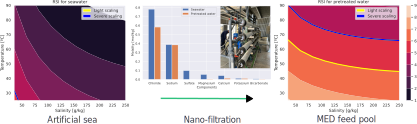
\includegraphics[]{figures/solarmed-std-tbt-pretreatment.png}
    \caption{\gls{rsiLabel} values as a function of temperature and concentration before (left) and after (right) pre-treatment using nanofiltration.}
    \labfig{solarmed:std:tbt-pretreatment}
\end{figure*}

\subsubsection{Monitoring and control system}
\labsec{solarmed:std:monitoring-control}

% Startup - shutdown FSMs
\textbf{Finite state machines}. Each day of operation requires starting up and shutting down the system, making it a repetitive and sufficiently complex process that requires an experienced operator. Manual management of the a process leads to errors that cause setbacks or, in the worst cases, premature failures in the facility: contamination of the condenser with brine due to erratic draining of the last effect, accumulation of scale on the surfaces of heat exchangers due to rapid cooling after shutdown, pumps cavitating because they are not stopped when the water flow at the intake ceases, etc. For this reason, two finite state machines have been implemented to manage the startup and shutdown of the facility. These have been designed to perform a sequence of operations that take the plant from an initial state to a final state following proper operating practices. A diagram of the process is shown in \reffig{solarmed:std:fsm}.

The machines are responsible for managing the activation and deactivation of devices as well as controllers. Additionally, they set reference values for these based on a previously established configuration and evaluate whether the reference has been reached before proceeding to the next step. They also adjust certain parameters of the control system (level control) and restore the initial values once the task is completed.

\begin{figure}
    \includegraphics[width=\textwidth]{figures/solarmed-std-startup_shutdown_fsm.png}
    \caption{Flowchart of finite state machines for plant start-up (left) and shutdown (right)}
    \labfig{solarmed:std:fsm}
\end{figure}

% On the other hand, before any of the processes begin, the status of various system variables is checked to ensure that they are available and, if so, that their values are compatible with startup/shutdown. If this is not the case, an alert is generated so that the variables can be addressed before another attempt is made.

In \reffig{solarmed:std:test-results} the activation sequence can be visualized at the beginning of the test (09:49--10:00): extractions $\rightarrow$ cooling $\rightarrow$ feedwater and heat source. The \textit{Flows} are activated in about two minutes followed by another minute for the inlet temperature. Then the system is left to stabilize. At 09:52 the delay between activating the feedwater and it reaching the last effect is completed and the brine extraction pump starts operating. Pressures, temperatures and the distillate level in the system progressively evolve up to 10:00 when the  conditions are changed for the first operation point for the day. The distillate level control action is delayed further until 10:04 when the first distillate is produced.   

Regarding the shutdown procedure, the two most delicate processes are the cooling of the first effect (which has the highest scaling potential if not done properly) and the complete draining of the last effect and condenser. For the gradual cooling of the first effect, after the plant shutdown signal, the hot water temperature is reduced in 5-minute steps starting from the last recorded value until a final temperature of 50°C is reached. To drain the levels, a reference value well below the normal operating level is set, and the controller parameters are changed to more aggressive ones. Additionally, the device is deactivated each time the reference is reached and is not reactivated until the level reaches a specified value. This activation and deactivation process continues while the feedwater finishes draining from the upper effects of the plant. Once the control system has been deactivated for longer than a preset time, the plant shutdown procedure is considered complete, and the level controller parameters are restored.

This procedure can be observed in \reffig{solarmed:std:test-results} starting from 13:07. After a decrease in flow rates, the first effect heat load is progressively decreased until 13:34. From this time, pumps are stopped and the extraction cycles begin as can be noted by the high oscillations in the \textit{Electrical consumption} -- $J_b$ and $J_d$ and \textit{Levels}.

% \begin{figure*}[h!]
%     \includegraphics[]{figures/med_20230418.png}
%     \savebox\captionqr{\qrcode[hyperlink,height=0.5in]{\repositoryBaseUrl/figures/med_20230418.html}}
%     \caption[]{Test results.\hspace{1ex}\usebox\captionqr}
%     \labfig{solarmed:std:test-results-20230418}
% \end{figure*}

\begin{figure*}
    \centering
    \subfloat[\centering
    Dynamic identification by means of PRBS signal]{{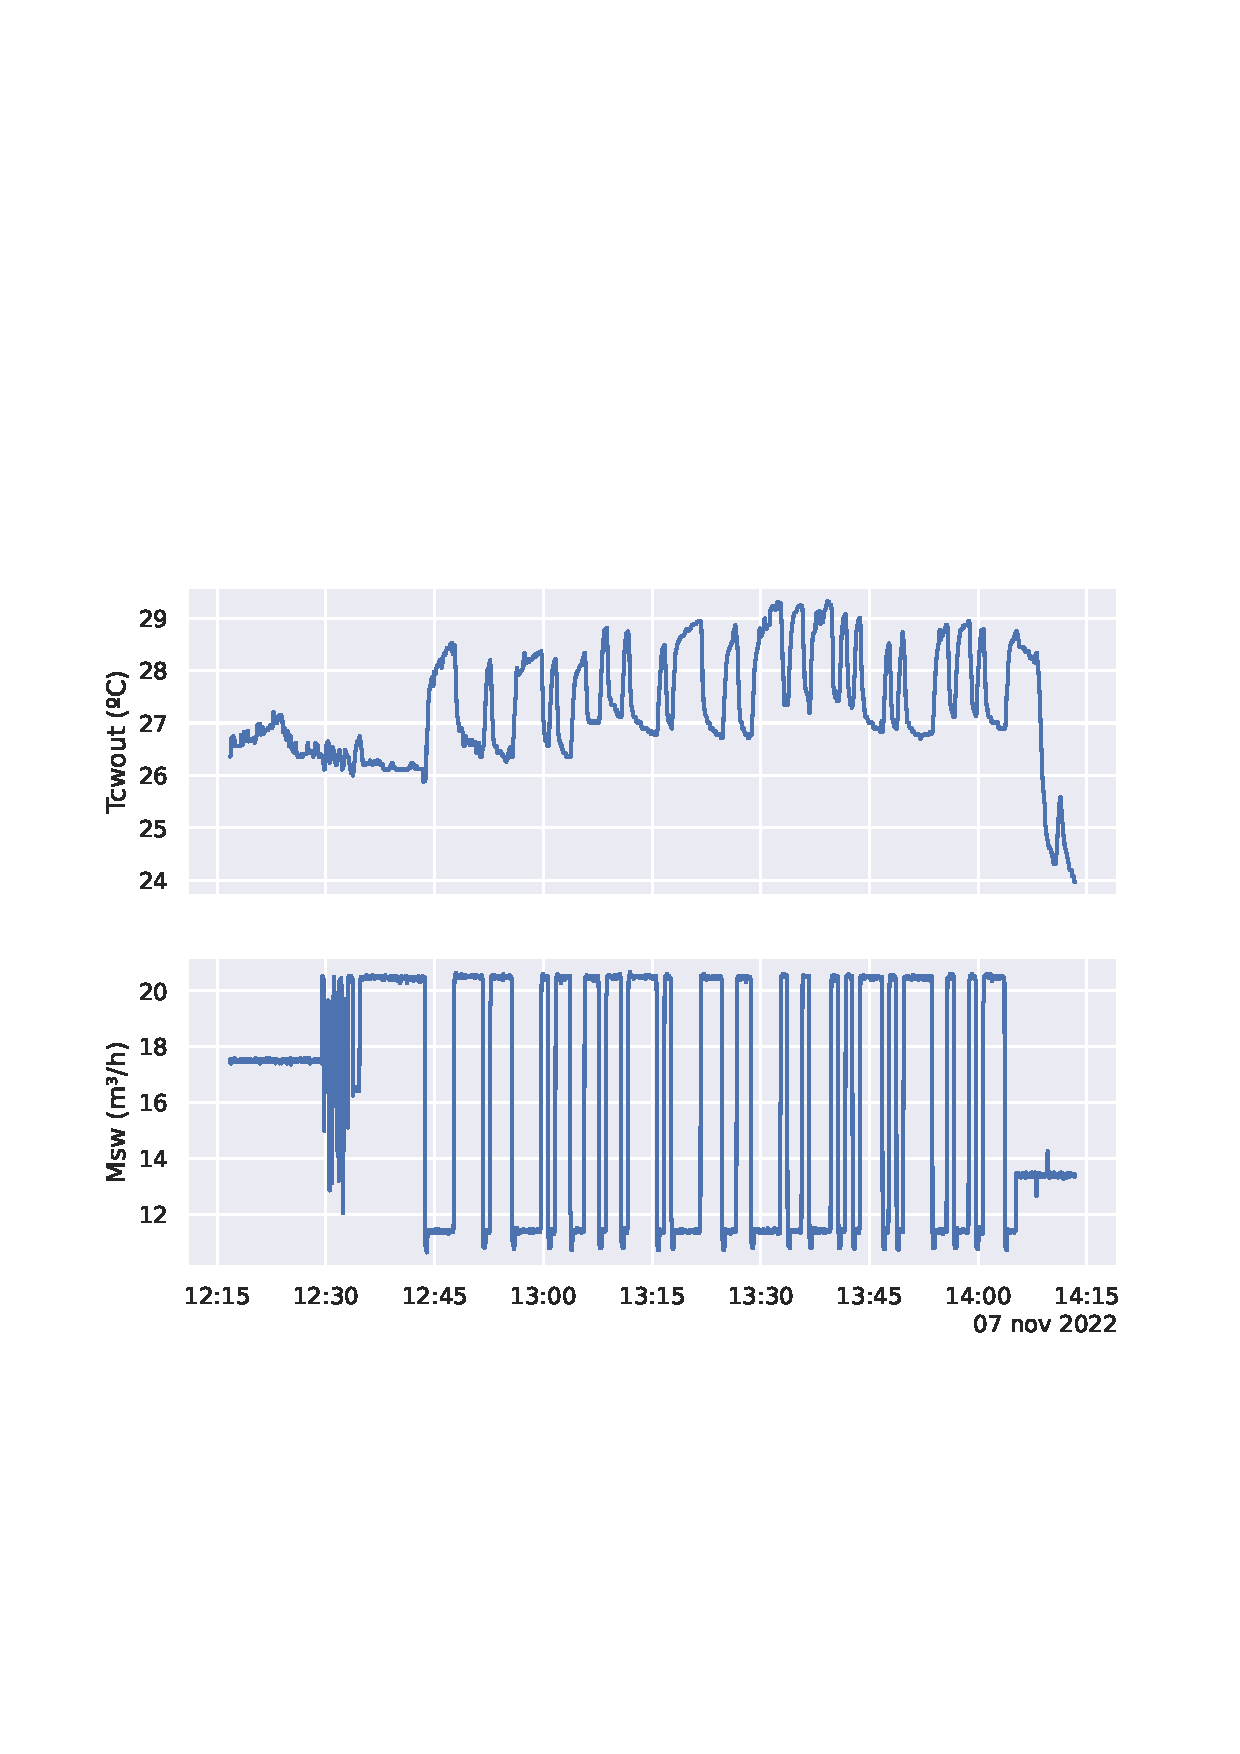
\includegraphics[width=0.48\linewidth]{figures/solarmed-std-control-tcout-ident.png}
    }}%
    \hspace{0.1cm}
    \subfloat[\centering
    Controller application results]{{\includegraphics[width=0.48\linewidth]{figures/solarmed-str-control-condenser_temperature.png}
    }}%
    \caption[Condenser outlet temperature controller implementation]{Condenser outlet temperature controller implementation. On (b) the perturbance (inlet temperature) is shown with a solid-green line, while the output (condenser outlet temperature) is shown with a solid-blue line. The reference is a thick dashed-green line.}
    \labfig{solarmed:std:condenser-control}
\end{figure*}

% Steady state identification
\textbf{Steady state identification}. The steady state identification algorithm has been implemented in the control system. It allows the automatic detection of stable operation points. This is done by monitoring the \glspl{kpvLabel} and applying the algorithm described in \refsec{solarmed:std:monitoring}. In \reffig{solarmed:std:test-results}, steady state periods are highlighted with a yellow background, which indicates that the algorithm has detected a stable operation point. Two are detected, the first one from 11:00 to 11:55 and the second one from 12:16 to 12:59.

% Controllers
\textbf{Control}. In terms of control, a \gls{pidLabel} control has been implemented to effectively regulate and maintain the desired setpoints of the subsystems mentioned in \refsec{solarmed:std:control}. This approach enables the system to respond quickly to changes, minimize steady state errors, reject disturbances, and enhance overall performance and reliability. \reffig{solarmed:std:condenser-control} shows the development procedure for one of the main loops, the condenser outlet temperature control. To tune the controller, the system was excited with a \gls{prbsLabel} signal (a), obtaining an ARX model ($n_a=20$, $n_b=49$, $n_k=5$, 96.38\% fit) using the \textit{System Identification Toolbox} from MATLAB, this allowed to extract an approximate first-order dynamic with which to tune the controller. \reffig{solarmed:std:condenser-control} (b) shows the controller performance for a particular test. Initially, the control signal ($q_c$) increases to compensate for the trend observed in the condenser inlet temperature. At 11:45 the setpoint\sidenote{\ie reference} is changed to 24 $^\circ$C, to which the controller inmediately adapts by decreasing its input and allowing the temperature to increase. The system progressively evolves towards the new setpoint, reached at 12:30 the controller then mantains the desired temperature compensating for other - not shown in the figure - disturbances. A similar situation can be observed in the showcased test of \reffig{solarmed:std:test-results} -- \textit{Temperatures} and \textit{Flows}. For the first operation point (11:00 onwards), the continuously increasing inlet temperature ($T_{c,in}$) is compensated by the controller, which increases the cooling flow rate to maintain the condenser outlet temperature at the setpoint. For the second operation point (12:16) the higher outlet temperature setpoint and turning on of the cooling tower allowing the inlet temperature to stabilize permits the controller to reduce the cooling flow rate and remain relatively unchanged.

\begin{figure*}[h!]
    \includegraphics[]{figures/med_20230508.png}
    \savebox\captionqr{\qrcode[hyperlink,height=0.5in]{\repositoryBaseUrl/figures/med_tests_viz.zip}}
    \caption[]{Test results. Several days available in interactive version \hspace{1ex}\usebox\captionqr}
    \labfig{solarmed:std:test-results}
\end{figure*}

\subsubsection{Reproducibility and the effect of the steady state duration}
\labsec{solarmed:std:results:reproducibility}
% 20230331 12:15 and 20230418 12:22: Duration from 16 to 76
% 20230329 13:10 and 20230414 12:51: Also the same test on different dates

The operation points pairs 1--2 and 3--4 in \reftab{solarmed:std:results} are the same test, \ie the same operating conditions, but performed on different days. Particularly for 1--2, the duration of the steady state is significantly different (16 and 76 minutes, respectively). The obtained performance metrics are similar, with almost identical values for the energectic and separation metrics. Slight differences, but still within the uncertainty margin are observed in metrics influenced by electrical consumption—which vary between tests due to differences in the cooling water inlet temperature: 17 (1) vs 13 (2) m$^3$/h for the cooling water flow rate, translates into a 0.3\% difference in second law efficiency and 0.1 KWh$_e$ for SEEC. Inlet condenser temperature conditions are more similar in 3--4 (22.6 vs 21.4 $^\circ$C), making differences for all metrics negligible.

Thus, it can be stated that the proposed methodology provides reproducible results and that the quality of stable operation and the ability to correctly identify it are of greater importance than the specific duration of the steady state.


% Tabla medidas de 8 puntos de operación (2 alta T, 2 baja T, 2 control, 2 con diferente duración de estacionario)
% Tabla de métricas de 8 puntos de operación

\begin{table*}[]
\caption{Measured variables and performance metrics for some operation points of the experimental campaign. The values are expressed as mean $\pm$ standard deviation with a coverage factor of 2 (95\% confidence interval). \textit{D} is the duration of the steady state period.}
\labtab{solarmed:std:results}

\resizebox{.9\linewidth}{!}{%
\begin{tabular}{ccccccccccccccccccccc}
\hline
\multirow{2}{*}{} &  & \multirow{2}{*}{\begin{tabular}[c]{@{}c@{}}\textbf{Test date}\\ (UTC)\end{tabular}} &  & \multirow{2}{*}{\begin{tabular}[c]{@{}c@{}}\textbf{D}\\ (min)\end{tabular}} &  & \multicolumn{14}{c}{\textbf{Performance metrics}} \\ \cline{7-20}
           &  &                 &  &                           &  & \begin{tabular}[c]{@{}c@{}}GOR\\ {\footnotesize (-) }\end{tabular} &  & \begin{tabular}[c]{@{}c@{}}STEC\\ {\footnotesize ($KW_{th}$) }\end{tabular} &  & \begin{tabular}[c]{@{}c@{}}SEEC\\ {\footnotesize ($KW_{e}$) }\end{tabular} &  & \begin{tabular}[c]{@{}c@{}}RR\\ {\footnotesize (-) }\end{tabular} &  & \begin{tabular}[c]{@{}c@{}}RI\\ {\footnotesize (-) }\end{tabular} &  & \begin{tabular}[c]{@{}c@{}}$\eta_{II}$\\ {\footnotesize (\%) }\end{tabular} &  & \begin{tabular}[c]{@{}c@{}}SEXC\\ {\footnotesize ($kWh_{ex}/m^3$) }\end{tabular} \\ \cline{3-3} \cline{5-5}\cline{7-7} \cline{9-9} \cline{11-11} \cline{13-13} \cline{15-15} \cline{17-17} \cline{19-19}
1 &   & 20230331 12:15 &   & 16 &   & $11 \pm 1$ &   & $60 \pm 6$ &   & $3.9 \pm 0.2$ &   & $29 \pm 1$ &   & $0.35 \pm 0.02$ &   & $8.0 \pm 0.6$ &   & $10.9 \pm 0.8$ &   \\
2 &   & 20230418 12:22 &   & 76 &   & $11 \pm 1$ &   & $59 \pm 6$ &   & $4.0 \pm 0.2$ &   & $29 \pm 2$ &   & $0.35 \pm 0.02$ &   & $7.7 \pm 0.6$ &   & $11.3 \pm 0.9$ &   \\
\cline{3-20}
3 &   & 20230329 13:10 &   & 24 &   & $10.1 \pm 0.7$ &   & $66 \pm 5$ &   & $3.9 \pm 0.2$ &   & $30 \pm 2$ &   & $0.35 \pm 0.02$ &   & $6.9 \pm 0.4$ &   & $12.7 \pm 0.8$ &   \\
4 &   & 20230414 12:51 &   & 27 &   & $10.2 \pm 0.7$ &   & $65 \pm 5$ &   & $3.9 \pm 0.2$ &   & $30 \pm 2$ &   & $0.36 \pm 0.02$ &   & $6.8 \pm 0.4$ &   & $12.8 \pm 0.8$ &   \\
5 &   & 20230511 11:23 &   & 32 &   & $8.1 \pm 0.4$ &   & $81 \pm 4$ &   & $3.2 \pm 0.2$ &   & $44 \pm 2$ &   & $0.52 \pm 0.02$ &   & $4.6 \pm 0.3$ &   & $17.8 \pm 0.9$ &   \\
\cline{3-20}
6 &   & 20230414 11:49 &   & 18 &   & $11 \pm 1$ &   & $59 \pm 5$ &   & $3.8 \pm 0.2$ &   & $47 \pm 3$ &   & $0.56 \pm 0.03$ &   & $7.2 \pm 0.5$ &   & $11.9 \pm 0.9$ &   \\
7 &   & 20230508 11:00 &   & 54 &   & $7.0 \pm 0.4$ &   & $93 \pm 6$ &   & $3.7 \pm 0.2$ &   & $48 \pm 3$ &   & $0.57 \pm 0.03$ &   & $3.9 \pm 0.3$ &   & $21 \pm 1$ &   \\
\hline
\end{tabular}
}

\bigskip

% TODO: Actualizar tabla con separadores
% TODO: Quitar la columna wd
% TODO: STEC y SEEC unidades están bien

\resizebox{\linewidth}{!}{%
\centering
\begin{tabular}{ccccccccccccccccccccccccc}
\hline
\multirow{2}{*}{} &  & \multicolumn{22}{c}{\textbf{Measured variables}} \\ \cline{3-24}
           &  & \begin{tabular}[c]{@{}c@{}}$T_{s,in}$\\ {\footnotesize (\si{\degreeCelsius}) }\end{tabular} &  & \begin{tabular}[c]{@{}c@{}}$T_{c,out}$\\ {\footnotesize (\si{\degreeCelsius}) }\end{tabular} &  & \begin{tabular}[c]{@{}c@{}}$q_{s}$\\ {\footnotesize (\si{\liter\per\second}) }\end{tabular} &  & \begin{tabular}[c]{@{}c@{}}$q_{f}$\\ {\footnotesize (\si{\cubic\meter\per\hour}) }\end{tabular} &  & \begin{tabular}[c]{@{}c@{}}$q_{d}$\\ {\footnotesize (\si{\cubic\meter\per\hour}) }\end{tabular} &  & \begin{tabular}[c]{@{}c@{}}$T_{s,out}$\\ {\footnotesize (\si{\degreeCelsius}) }\end{tabular} &  & \begin{tabular}[c]{@{}c@{}}$T_{c,in}$\\ {\footnotesize (\si{\degreeCelsius}) }\end{tabular} &  & \begin{tabular}[c]{@{}c@{}}$w_{f}$\\ {\footnotesize (\si{\milli\siemens\per\centi\meter}) }\end{tabular} &  & \begin{tabular}[c]{@{}c@{}}$w_{d}$\\ {\footnotesize (\si{\micro\siemens\per\centi\meter}) }\end{tabular} &  & \begin{tabular}[c]{@{}c@{}}$q_{c}$\\ {\footnotesize (\si{\cubic\meter\per\hour}) }\end{tabular} &  & \begin{tabular}[c]{@{}c@{}}J\\ {\footnotesize (\si{\kilo\watt}) }\end{tabular} \\ \cline{3-3} \cline{5-5} \cline{7-7} \cline{9-9} \cline{11-11} \cline{13-13} \cline{15-15} \cline{17-17} \cline{19-19} \cline{21-21} \cline{23-23}
1 &   & $64.0 \pm 0.8$ &   & $28.1 \pm 0.6$ &   & $12.0 \pm 0.2$ &   & $8.0 \pm 0.1$ &   & $2.4 \pm 0.1$ &   & $61.1 \pm 0.7$ &   & $24.5 \pm 0.7$ &   & $67.4 \pm 0.7$ &   & $8.00 \pm 0.08$ &   & $17 \pm 1$ &   & $\left(8.0 \pm 0.2\right) \times 10^{3}$ &   \\
2 &   & $64.0 \pm 0.7$ &   & $28.0 \pm 0.6$ &   & $12.0 \pm 0.3$ &   & $8.0 \pm 0.1$ &   & $2.3 \pm 0.1$ &   & $61.2 \pm 0.7$ &   & $23 \pm 1$ &   & $67.4 \pm 0.7$ &   & $8.00 \pm 0.08$ &   & $13 \pm 2$ &   & $\left(8.1 \pm 0.2\right) \times 10^{3}$ &   \\
\cline{3-24}
3 &   & $68.0 \pm 0.7$ &   & $28.0 \pm 0.6$ &   & $12.0 \pm 0.2$ &   & $8.0 \pm 0.1$ &   & $2.4 \pm 0.1$ &   & $64.8 \pm 0.7$ &   & $22.6 \pm 0.6$ &   & $67.4 \pm 0.7$ &   & $8.00 \pm 0.08$ &   & $13.8 \pm 0.8$ &   & $\left(8.1 \pm 0.2\right) \times 10^{3}$ &   \\
4 &   & $68.0 \pm 0.7$ &   & $27.9 \pm 0.8$ &   & $12.0 \pm 0.3$ &   & $8.0 \pm 0.1$ &   & $2.4 \pm 0.1$ &   & $64.8 \pm 0.6$ &   & $21.4 \pm 0.8$ &   & $67.4 \pm 0.7$ &   & $8.00 \pm 0.08$ &   & $10.9 \pm 0.9$ &   & $\left(8.1 \pm 0.2\right) \times 10^{3}$ &   \\
5 &   & $88.9 \pm 0.9$ &   & $29 \pm 1$ &   & $12.0 \pm 0.3$ &   & $7.0 \pm 0.1$ &   & $3.1 \pm 0.1$ &   & $83.8 \pm 0.9$ &   & $22 \pm 1$ &   & $64.7 \pm 0.6$ &   & $8.00 \pm 0.08$ &   & $20.1 \pm 0.3$ &   & $\left(7.9 \pm 0.3\right) \times 10^{3}$ &   \\
\cline{3-24}
6 &   & $68.0 \pm 0.7$ &   & $28.0 \pm 0.5$ &   & $12.0 \pm 0.3$ &   & $5.0 \pm 0.1$ &   & $2.4 \pm 0.1$ &   & $65.2 \pm 0.7$ &   & $20.8 \pm 0.6$ &   & $67.4 \pm 0.7$ &   & $8.00 \pm 0.08$ &   & $10.1 \pm 0.4$ &   & $\left(7.9 \pm 0.3\right) \times 10^{3}$ &   \\
7 &   & $89.0 \pm 0.7$ &   & $28.1 \pm 0.6$ &   & $12.0 \pm 0.3$ &   & $5.0 \pm 0.1$ &   & $2.4 \pm 0.1$ &   & $84.4 \pm 0.8$ &   & $21 \pm 2$ &   & $64.5 \pm 0.7$ &   & $8.00 \pm 0.08$ &   & $16 \pm 3$ &   & $\left(7.8 \pm 0.3\right) \times 10^{3}$ &   \\
\hline
\end{tabular}
}

\end{table*}

% \begin{table*}[]
% \caption{Performance metrics for some operation points of the experimental campaign. The values are expressed as mean $\pm$ standard deviation with a coverage factor of 2 (95\% confidence interval). \textit{D} is the duration of the steady state period.}
% \labtab{solarmed:std:performance-metrics}
% \resizebox{\linewidth}{!}{%
% }
% \end{table*}

%================================
\subsection{Results analysis}

% When the system was planned, it was designed to optimize for \textit{seawater desalination} and considering \textit{process heat}\sidenote{See \refsec{solarmed:std:process}} as the only external thermal energy source. 

%This is reflected in the higher performance values that can be observed, with low temperature difference between inlet and outlet of the heat source, whereas for brine concentration low recoveries are observed, and poor performance values are observed for the waste heat metrics

% \subsubsection{Best operating strategy}

% One caveat of the exergetic metrics for this particular plant, where the sink\sidenote{the simulated-fixed volume seawater} can change its conditions with significant dynamics, is that otherwise similar operating points can have different exergetic performance due to the additional cooling consumption required to maintain a certain condenser pressure / condenser outlet temperature. In order to enable fair comparison of the exergetic performance of different operating points, the cooling consumption is normalized to seawater intake at 20 $^\circ$C. 

% \subsubsection{Experimental evaluation at high \glspl[format=long]{tbtLabel}}

In \reftab{solarmed:std:results} operation points 4-5 and 6-7 compare low and high \gls{tbtLabel} operation. Two of them (4 and 6) receive heat at 68$^\circ$C, while they differ in the feedwater flow rate ($q_f$), one (4) with a higher value (8 m$^3$/h) and the other (6) at a lower one (5 m$^3$/h). The other two operation points receive heat at 89$^\circ$C and similar feedwater flow rate\sidenote{Equal between 4 and 5, slightly different but comparable between 6 and 7}. The first two operation points result in an approximate \gls{tbtLabel} of 61.5$^\circ$C while the last two operation points have an approximate \gls{tbtLabel} of 79.2$^\circ$C. This operation points selection is made to compare the performance of the plant at low and high \gls{tbtLabel} operation with otherwise equivalent conditions.

\textbf{Performance analysis}. The first immediate observation is that contrary to what stated in the introduction, the performance of the plant does not improve with higher heat source temperatures, on the contrary it decreases: \gls{gorLabel} -20\% and -36\% for the low (4-5) and high (6-7) $q_f$ scenario, respectively. Results are even worse in in terms of second law efficiency: -32\% and -46\%, respectively, since higher quality heat is being being destroyed. In summary, more energy, of better quality is being consumed to produce distillate less eficiently\todo{comprobar números}.

This can be explained by the fact that the increase in the heat source temperature is not taken advantage of by introducing more effects, which would provide the increase in efficiency.

On the other hand, the concentration achieved does increase significantly for the high $q_f$ scenario, with a 47\% increase in the recovery ratio. This is not the case for the low $q_f$ scenario, where the recovery ratio is similar to the low temperature operation point. A possible explanation is presented hereinafter.

\begin{figure}
    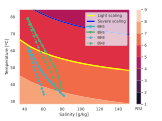
\includegraphics[width=.8\textwidth]{figures/solarmed-std-tbt-results.png}
    \caption{Temperature and concentration evolution for operation points at each effect in the \gls{medLabel} plant. Surface represents the \gls{rsiLabel}.}
    \labfig{solarmed:std:tbt-results}
\end{figure}

Using a physical model of the plant\sidenote{A detailed description of the model can be found in the
Appendix, \nrefch{appendix:med-model}}, a better insight into the inner working of the plant can be obtained. The model is based on the energy and mass balances of the system, and it is used to estimate different outputs at the effect level, such as the temperature and pressure of the vapor, the distillate production, and the brine concentration. This allows to analyze the temperature and concentration evolution and visualize it as shown in \reffig{solarmed:std:tbt-results}. According to the \gls{rsiLabel}, the high temperature operation points (5, 7) do get into the light scaling zone for the first 7 effects, while the low temperature operation points (4, 6) remain in the stable water zone for all effects.

\begin{figure*}[h!]
    \subfloat[\centering
    Energy contribution. Number in brine bar represents percentage of energy absorbed by it]{{\includegraphics[width=0.48\linewidth]{figures/med-tbt-energy-comp-68_28_12_5-20230414_vs_89_28_12_5-20230508.png}
    }}%
    \hspace{0.1cm}
    \subfloat[\centering
    Vapor generated. Value in bar represents flashing percentage]{{\includegraphics[width=0.48\linewidth]{figures/med-tbt-vap-gen-comp-68_28_12_5-20230414_vs_89_28_12_5-20230508.png}
    }}%
    \caption{Per effect comparison between low and high \gls{tbtLabel} operation points}
    \labfig{solarmed:std:tbt-analysis}
\end{figure*}

A per effect comparison can also be made in terms of energy contribution for vapor generation. This is shown in \reffig{solarmed:std:tbt-analysis} (a) for the low $q_f$ scenario. In the first effect a stark difference between low and high operation can be seen, with almost double the power released, producing almost double the vapor (\reffig{solarmed:std:tbt-analysis} -- (b)). However this difference is not maintained in the following effects, but an opposite trend is observed. Effect 8 is the crossing point and from there on the low temperature operation point produces more vapor. Another interesting comparison is the \textit{mixer} energy contribution, the higher temperature of the distillate produced in the first effects becomes a signficant contributor in the later effects, with a greater impact compared to the low temperature operation. Thus, distillate distribution is more effective when total plant temperature differences are higher. 

An explanation as to why vapor generation seems limited and thus the achieved concentration, can be the \gls{bpeLabel} of the brine (see \reffig{solarmed:std:tbt-analysis} (b)), which is a function of temperature and concentration, increasing with the latter. This means that the temperature difference between the brine and the vapor is reduced, and, which in turn reduces the boiling driving force. In the visualized case, the final \gls{bpeLabel} value for the low-temperature operation is reached by effect 9 of the high temperature one. In an  \gls{medLabel}  plant, the vapor generated in the previous effect is the driving force for the next effect (\reffig{solarmed:std:tbt-analysis} -- (a)), low vapor production on one effect means a diminished force for heat transfer in the next one, which in turn reduces the vapor production on that effect. It is an exponential decay process. That is why despite the larger energy availability in the first effects, the better balaced effects of the low temperature operation turns out to ultimately produce similar levels of separation~\sidecite{lienhardv_energy_2019}.

In this figure, it can be seen than flashing takes a more relevant role in vapor generation in the latter effects of the high temperature alternative, since it is not affected by \gls{bpeLabel} (8,9 and 17\% of the total vapor generated in effects 12, 13 and 14, respectively). This indicates that maybe flashing is a good alternative to increase the vapor production in the latter stages of a thermal brine concentrator plant. 

\begin{remark}
    A MED-MSF hybrid could be a good alternative to increase the brine concentration in the last effects, where the vapor production is limited by the \gls{bpeLabel}. Another option worth exploring is variable geometry effects, in order to increase temperature differences and mantain vapor production at higher concentrations.
\end{remark}

\textbf{Scaling assessment}. To assess whether scaling occurred during high-temperature operation, control tests were conducted both before the high-temperature tests and repeated after about 30 hours of operation. In \reftab{solarmed:std:results} the same operation points used to validate the reproducibility \sidenote{\nrefsec{solarmed:std:results:reproducibility}}, \ie: 1-2 and 3-4 can be used to draw conclusions. Aside from the mentioned differences in metrics influenced by electrical consumption, the performance metrics values are consistent across tests, suggesting that the system is operating efficiently without significant fouling or scaling.\todo{Incluir una gráfica de los coeficientes de transferencia para ambos tests?}

% \textbf{Conclusions}.

% \section{Conclusion}

% Sobre las métricas

% Sobre la metodología

% Sobre los resultados a alta temperatura

